\section{Solution} \label{sec:solution}
The solution we propose to the problem statement, introduced in the introduction, is as follows:
\begin{itemize}
	\item	Input a payload description file that specifies all of the payloads, and input some parameters that specifies the environment and validation options
	\item	Produce a \gls{cora} model that will find the a near optimal schedule in regards to profit while guaranteeing the battery level will never fall below a certain level
	\item	Validate the schedule in \gls{smc} to test the robustness and act accordingly to the result as well as getting a more accurate simulation of the battery consumption
	\begin{itemize}
		\item	Rejected: modify the input and produce a new schedule for validation
		\item	Accepted: output schedule along with relevant values
	\end{itemize}
\end{itemize}

By doing so we are able to produce a schedule that schedules the payloads and is verified in regards to the robustness.
How the schedule is generated and how the robustness is tested will be explained in the following chapters of this report.
Prior to defining the input language in \cref{sec:read_input} \nameref{sec:read_input}, we will present our tool-chain which provides an overview of how the final system will work and how the different tools are used.

\subsection{Tool-chain} \label{subsec:tool_chainv}
In order to clarify our usage of different tools we will describe the different steps in our system. 
\Cref{fig:tool1} displays a flowchart representation of the tool-chain.

\begin{figure}[h]
	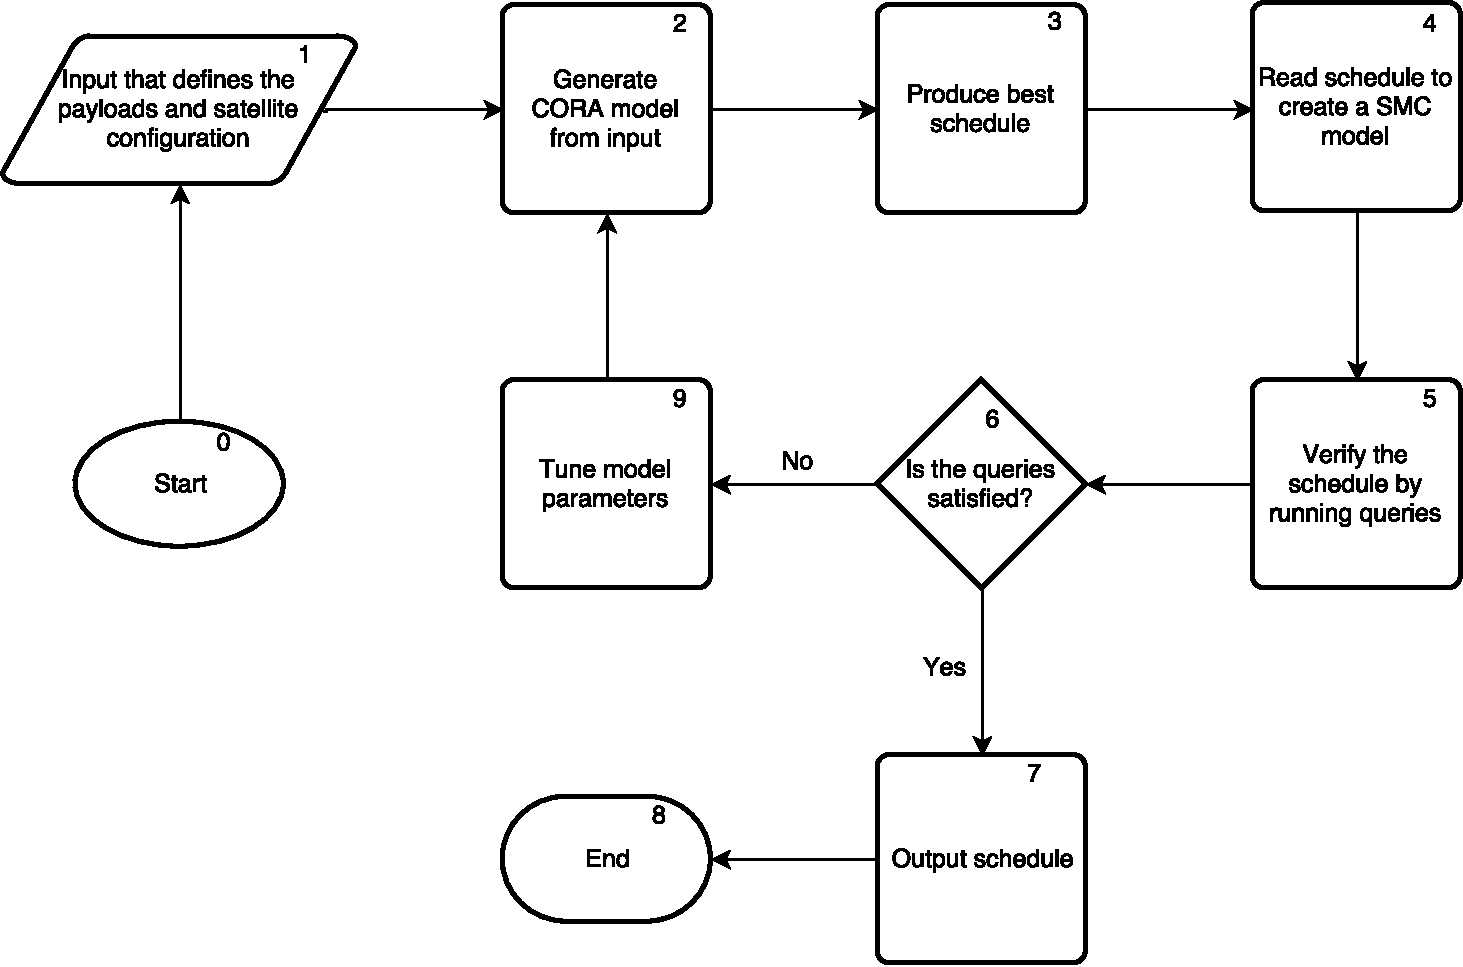
\includegraphics[width=\textwidth]{graphics/flow_final.pdf}
	\caption{Flowchart that displays the workflow and use of tools}
	\label{fig:tool1}
\end{figure}

\paragraph{Location 1 - CSV file that contains payload information} 
Is the input file for the system. 
The usage of this file and its format is described in \cref{sec:read_input}.

\paragraph{Location 2 - Generate \gls{cora} XML models file from input} 
In this location we will read the CSV file or the tuned parameters from location 9. 
The input is used to generate two \gls{cora} models.
The values specified in the input file can be in a range to indicate variations or uncertainties in how much time, power, etc. a payload uses.
One model uses the worst case values and the other will use the interval. 

%\paragraph{Location 3 - Input model to CORA Verifyta} the Verfyta will generate a trace for each model.

\paragraph{Location 4 - Test worst case model} 
Run the queries on the worst case model.

\paragraph{Location 5 - Is the worst case possible?} 
If we were unable to produce a trace for the worst case, we will not be able to guarantee that any of the schedules we produce will stay within the specified parameters. 
We will as a result thereof go to location 6, the fail state.

\paragraph{Location 7 - Extract trace from the \gls{cora} model and it to \acrshort{lbtp}} 
In this location we will extract a trace from the \gls{cora} model and use it as input for the tracer function in \acrshort{lbtp}. 
The tracer function will transform the output into a readable trace which can be used later on.

%\paragraph{Location 9 - Convert trace to \gls{smc} xm model file} in this location we will read the trace and produce the \gls{smc} model that will be used in the next location.

\paragraph{Location 10 - Verify queries and extract the results} 
The \gls{smc} Verifyta will run the queries on the \gls{smc} model and output the results, see \cref{sec:smc}. 
These queries is made to validate and test the robustness of the trace.

\paragraph{Location 13 - Output schedule} 
If the queries are satisfied we will output the schedule, as this will indicate that the trace, or schedule, is correct.

\paragraph{Location 12 - Tune model parameters} 
If the queries were not satisfied, the schedule will be discarded and we will produce a new one. 
In order to produce a new schedule, we will provide \gls{cora} with a new set of parameters based on those from the CSV file. 
These parameters will be loyal to those specified in the CSV file, but their ranges will be shortened in order to provoke new choices in the schedule. 
This will change the workflow as we are not interested in verifying the worst case model any more, as the previous worst case is still true to this version of the parameters. 
We will therefore skip location 4, 5, and 6 and will go directly yo location 7.

